
\documentclass[a4paper,12pt]{report}
\usepackage{latexsym}
\usepackage[MeX]{polski}
\usepackage[utf8]{inputenc}	% kodowanie znaków
\usepackage{listings} 		% kolorowanie składni
\usepackage{color}		% kolory
\usepackage{xcolor}		% bonusowe kolory
\usepackage{hyperref}	% linki w spisie treści, odnośniki, zakładki w pdf
\usepackage{upquote}  	% zamiana cudzysłowów klasycznych (,, ") na górne (" ") w kodach źródłowych
\usepackage{graphicx}	% wskawianie obrazków

% Ustawienie marginesów
\oddsidemargin=0cm
\topmargin=0cm
\textwidth=16cm
\textheight=23cm

% Ustawienie ładnych etykiet do kodów źródłowych
\usepackage{caption}		
\DeclareCaptionFont{white}{\color{white}}
\DeclareCaptionFormat{listing}{\colorbox{gray}{\parbox{\textwidth}{#1#2#3}}}
\captionsetup[lstlisting]{format=listing,labelfont=white,textfont=white}


%Zdefiniowanie autora i~tytułu:
\author{Kacper Szkudlarek, Maciej Stefańczyk}
\title{PUCY MP\_02}

\frenchspacing


%%
%% AHDL definition
%%
\lstdefinelanguage{AHDL}%
  {morekeywords={AND,BEGIN,BIDIR,BITS,BURIED,CARRY,CASCADE,CASE,CLIQUE,CONNECTED_PINS,CONSTANT,
DEFAULTS,DESIGN,DEVICE,DFF,DFFE,ELSE,ELSIF,END,EXP,FUNCTION,GLOBAL,GND,IF,INCLUDE,INPUT,IS,JKFF,JKFFE,
LATCH,LCELL,MACHINE,MACRO,MCELL,NAND,NODE,NOR,NOT,OF,OPTIONS,OR,OTHERS,OUTPUT,RETURNS,SRFF,SRFFE,
SOFT,STATES,SUBDESIGN,TABLE,TFF,TFFE,THEN,TITLE,TRI,VARIABLE,VCC,WHEN,WITH,X,XNOR,XOR},% 
   sensitive=f,
   morecomment=[l]--,%
   morecomment=[s]{\%}{\%},%
   morestring=[d]{"}%
  }[keywords,comments,strings]%

\lstdefinelanguage{oasm}%
  {morekeywords={STOP, RESET, JMP, JZ, ADD, SUB, LD, OR, AND, LDI, IN, OUT, STORE, MUL},%
   sensitive=f,%
   morecomment=[l];,% nonstandard
  }[keywords,comments]%

\lstset{
	language=,	                		% choose the language of the code
	basicstyle=\footnotesize\ttfamily,       	% the size of the fonts that are used for the code
	numbers=left,                   		% where to put the line-numbers
	numberstyle=\tiny,      			% the size of the fonts that are used for the line-numbers
	stepnumber=1,                   		% the step between two line-numbers. If it's 1 each line will be numbered
	numbersep=5pt,                  		% how far the line-numbers are from the code
	showspaces=false,               		% show spaces adding particular underscores
	showstringspaces=false,         	% underline spaces within strings
	showtabs=false,                 		% show tabs within strings adding particular underscores
	tabsize=4,	                		% sets default tabsize
	captionpos=t,                   		% sets the caption-position
	breaklines=true,                		% sets automatic line breaking
	breakatwhitespace=true,        	% sets if automatic breaks should only happen at whitespace
	extendedchars=true,
	keywordstyle=\color{blue}\bfseries,
	commentstyle=\color{gray}\textit,
}

\begin{document}

%Wstawienie autora i~tytułu do składu:
\maketitle

%Wstawienie spisu treści:
\tableofcontents



%%%%%%%%%%%%%%%%%%%%%%%%%%%%%%%%%%%%%%%%%%%%%%%%
% Wiadomości ogólne o całym projekcie
%%%%%%%%%%%%%%%%%%%%%%%%%%%%%%%%%%%%%%%%%%%%%%%%
\chapter{Realizacja ogólna}

\section{Treść zadania}

Zadanie polegało na zaprojektowaniu 8-bitowego mikrokontrolera ogólnego przeznaczenia, wyposażonego w kilka wbudowanych podzespołów (pamięć ROM, pamięć RAM, układ wejściowy wczytujący dane z klawiatury, układ wyjściowy drukujący dane na drukarce) oraz umożliwiającego podłączanie kolejnch podzespołów poprzez wyprowadzoną na zewnątrz szynę systemową. Bloki funkcjonalne mikrokontrolera powinny być zaprojektowane jako niezależne elementy współpracujące ze sobą za pośrednictwem wewnętrznej, trójstanowej szyny systemowej.

\section{Założenia projektowe}
Dane wejściowe i wyjściowe wprowadzane i wypisywane są w postaci 4 znaków ASCII w postaci ZDDD, wyznaczających wartość dziesiętną ze znakiem z przedziału [-128, +127]. Dane na wejściu podawane są bez błędów, jednak mimo tego zabezpieczyliśmy się przed podaniem liczb spoza zakresu.

\subsubsection{Zestaw instrukcji}
Procesor powinien obsługiwać następujący zestaw poleceń: (patrz też:~\ref{sec:asmex})
\begin{itemize}
\item Instrukcje sterujące
\begin{description}
\item[STOP] \hfill \\
Zatrzymanie wykonywania programu, wyjście z tego stanu możliwe jedynie przez reset układu.
\item[RESET] \hfill \\
Powrót programu do pierwszej instrukcji. $PC <= 0$
\item[JMP A] \hfill \\
Skok bezwarunkowy pod adres A (8 bitów). $PC <= A$
\item[JZ Rd A] \hfill \\
Skok warunkowy pod adres A. $Rd == 0 => PC <= A$
\end{description}

\item Operacje arytmetyczne i logiczne
\begin{description}
\item[ADD Rd, Ra, Rb] \hfill \\
Dodawanie. $Rd <= Ra + Rb$
\item[SUB Rd, Ra, Rb] \hfill \\
Odejmowanie. $Rd <= Ra - Rb$
\item[MUL Rd, Ra, Rb] \hfill \\
Mnożenie (wykonywane metodą Bootha). $Rd <= Ra * Rb$
\item[AND Rd, Ra, Rb] \hfill \\
Iloczyn bitowy. $Rd <= Ra and Rb$
\item[OR Rd, Ra, Rb] \hfill \\
Suma bitowa. $Rd <= Ra or Rb$
\end{description}

\item Operacje na pamięci oraz wejścia/wyjścia
\begin{description}
\item[LDI Rd, D] \hfill \\
Załadowanie wartości do rejestru Rd. $Rd <= D$
\item[LD Rd, Ra, Rb] \hfill \\
Wczytanie danych z pamięci spod adresu wskazywanego przez rejestry Ra i Rb. $Rd <= (RaRb)$
\item[STORE Rd, A] \hfill \\
Zapisanie zawartości rejestru Rd do pamięci pod adres A (16-bitowy). $Rd => (A)$
\item[IN Rd, A] \hfill \\
Wczytanie do rejestru Rd danych z urzadzenia wejściowego o adresie A (8-bitowy). $Rd <= IN(A)$
\item[OUT Rd, A] \hfill \\
Wyprowadzenie zawartości rejestru Rd do urzadzenia wyjściowego o adresie A (8-bitowy). $Rd => OUT(A)$
\end{description}

\end{itemize}

Wszystkie operacje wykonywane są na liczbach 8-bitowych zapisanych w kodzie U2.

Mikrokontroler posiada 8 rejestrów ogólnego przeznaczenia (R0..R7).

\subsubsection{Szyna systemowa}

Szyna systemowa składa się z 3 grup sygnałów: linii adresowych (16 bitów), linii danych (8 bitów) oraz sygnałów sterujących, które dokładniej opisane są niżej.
\begin{description}
\item[/RD] Sygnał żądania odczytu danych
\item[/WR] Sygnał żądania zapisu danych
\item[/MREQ] Sygnał żądania dostępu do przestrzeni adresowej pamięci (16 bitów)
\item[/IOREQ] Sygnał żądania dostępu do przestrzeni adresowej wejścia/wyjścia (8 bitów)
\item[WT] Sygnał oczekiwania sygnalizujący trwającą operację, procesor powinien zaczekać
\end{description}

Dodatkowo do każdego komponentu doprowadzone są sygnały GEN (zegar systemowy 40MHz) oraz CR (asynchroniczne zerowanie układu).

\section{Schemat blokowy układu}

Na rysunku~\ref{fig:block} przedstawiony został schemat blokowy zaprojektowanego układu. Każdy bloczek oznacza w ogólnosci pojedynczy moduł systemu (zaprojektowany osobno i niezależnie od pozostałych). Bloczki zawarte wewnątrz innych są ich częścią składową i poza nimi nie ma do nich dostępu (np. blok mnożenia i rejestry CPU, zamiana postaci U2 na format BCD w układzie wyjściowym).

\begin{figure}[h]
\centering
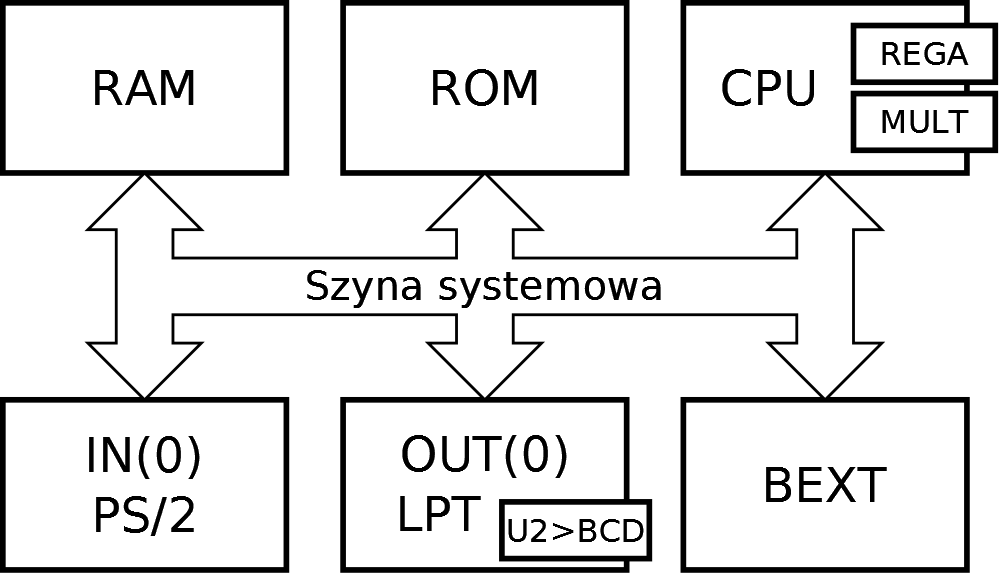
\includegraphics[width=8cm]{./pict/Block.png}
\caption{Ogólny schemat blokowy projektowanego układu.}
\label{fig:block}
\end{figure}

%%%%%%%%%%%%%%%%%%%%%%%%%%%%%%%%%%%%%%%%%%%%%%%%
% Dokładne opisy poszczególnych komponentów
%%%%%%%%%%%%%%%%%%%%%%%%%%%%%%%%%%%%%%%%%%%%%%%%
\chapter{Opis komponentów}

\section{Moduł CPU}


\subsection{Wczytywanie instrukcji, operandów i rejestrów}
Główny moduł mikrokontrolera został zaimplementowany w postaci jednej maszyny stanów, której poszczególne stany są dokładniej omówione w dalszj części opisu. Przy projektowaniu została podjęta decyzja, że zamiast warunkowego pobieraniadrugiego i ewentualnie trzeciego bajtu z pamięci w zależności od instrukcji, a także od warunkowego pobierania wartości z rejestrów, zawsze będą pobierane 3 słowa z pamięci i odczytywane trzy rejestry. Działa to w sposób następujący:
\begin{itemize}
  \item Z pamięci odczytywane jest pierwsze słowo (zawierające kod rozkazu i ewentualnie numer rejestru)
  \item Z pamięci odczytywane jest drugie słowo, a jednoczeście do zmiennej pomocniczej wczytywana jest zawartość rejestru o numerze zakodowanym w pierwszym słowie
  \item Z pamięci wczytywane jest trzecie słowo, a z rejestrów wczytywane są te o numerach zakodowanych w drugim słowie
\end{itemize}
W ten sposób zawsze do trzech zmiennych IC1..IC3 wczytywane są trzy słowa z pamięci programu, a do zmiennych TMP0..TMP2 wczytywana jest zawartość trzech rejestrów. Dzięki temu w późniejszym etapie przy wykonywaniu instrukcji wszystkie potrzebne dane są już przygotowane i wykonanie operacji najczęściej sprowadza się do zapisania wyniku do pamięci i odpowiedniego zwiększenia licznika rozkazów PC. Jeśli instrukcja, którą obsługujemy jest krótsza niż 3 słowa (a większość jest), to po zwiększeniu PC "niewykorzystane" słowa zostaną ponownie wczytane i zinterpretowane przez następną komendę. 

Niewątpliwą zaleta takiego rozwiązania jest duże uproszczenie funkcji każdej instrukcji, przy poświęceniu niewiele dłuższego czasu na obsługę całego cyklu (różnica jest praktycznie niezauważalna, a w niektórych przypadkach rozwiązanie zastosowane przez nas jest szybsze od pobierania kolejnych słów instrukcji i wczytywania zawartości rejestrów już w funkcji obsługi danej instrukcji).

\subsection{Opis stanów procesora}
Pojedynczy cykl pracy procesora, a więc przejście od wczytania instrukcji i operandów aż do jej wykonania i zapisania wyników, moze wymagać przejścia przez następujące stany:
\begin{description}
\item[ST0] \hfill \\
Sprawdzenie, czy nie został ustawiony sygnał STOP (poprzez wykonanie instrukcji STOP bądź niedozwoloną sekwencję sterującą), oraz pobranie z pamięci słowa spod adresu wskazywanego przez PC.
\item[ST1] \hfill \\
Odczekanie ustalonej liczby taktów na ustalenie się danych odczytanych z pamięci\footnote{Podczas testów okazało się, że pamięć nie nadąża z ustawieniem danych na liniach, przez co procesor dostawał błędne odczyty}
\item[ST2] \hfill \\
Zapisanie danych do odpowiednich zmiennych pomocniczych (dane wczytane z pamięci do zmiennych IC1..IC3, wczytanie zawartości odpowiednich rejestrów do zmiennych TMP0..TMP2)
\item[ST3] \hfill \\
Interpretacja oraz wykonanie instrukcji wczytanej z pamięci. Wszystkie operandy sa już wczytane, a więc w większości przypadków wymagane jest jedynie zapisanie wyniku odpowiedniego działania do pamięci bądź do rejestru. W przypadku operacji wymagających odczekania na sygnał WAIT jest to realizowane już wewnątrz danego bloku instrukcji.
\item[ST\_WAIT] \hfill \\
Stan oczekiwania przed rozpoczęciem nowego cyklu pracy, wykorzystywany podczas zapisu wyników wykonania poprzedniej instrukcji do pamięci.
\end{description}

\section{Pamięci wewntętrzne}
Do realizacji pamieci wewnętrznych zostyały wykorzystane moduly zawarte w  bobliotece LPM firmy Altery. Bilbioteka zawiera konfigorowalne definicje podtsawowych, najczęściej używanych bloków funkcjonalnych, które można zrealizować na układach FPGA.

\subsection{Pamięć RAM}
Do realizacji pamieci RAM został użytu moduł lpm\_ram\_dq. Jest to pamieć RAM z rozdzielonym wejściem i wyjściem. Może być używana jako pamięć synchroniczna lub asynchroniczna. W projekcie pamieć została zdefiniowana jako synchroniczna. Synchronizowany jest dostęp do danych, jak i szyny adresowej. Sygnałem synchronizującym operacje zapisu i odzcytu danych jest zegar systemowy. Ponieważ szyna danych, do której podłączny jest moduł, jest trójstanowa, niezbędne było także takie skonfigurwowanie elementy, by w momencie, gdy nie jest odpowiednio wysterowany do pracy, pozostawiał szynę danych wolną dla innych modułów.

\begin{figure}[h]
\centering
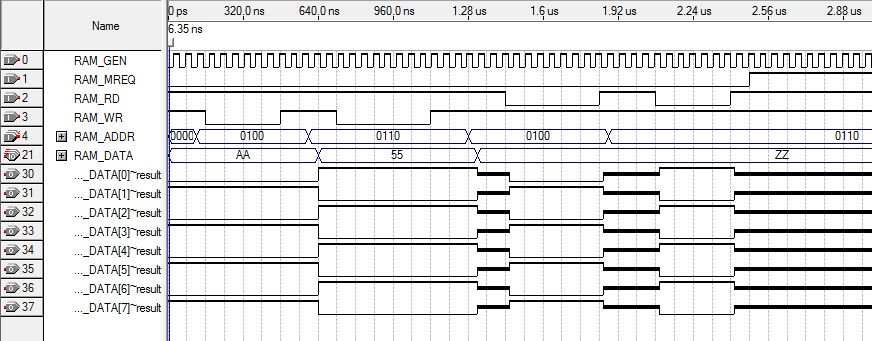
\includegraphics[width=15cm]{./pict/ram.jpg}
\caption{Przebiegi czasowe na poszczególnych liniach modułu pamięci RAM.}
\label{fig:ram}
\end{figure}

\subsection{Pamięć ROM}
Pamięć ROM równierz w oparciu o moduł z bibliteki LPM - lpm\_rom. Moduł może być używany zarówneo  jako pamięć synchroniczna i asynchroniczna. W projekcie pamieć zostałą użyta w postaci asynchronicznej. Sterowany jest jedynie dostęp modułu do trójstanowej szyny danych. W momencie, gdy nie następuje odczyt danych, moduł przechodzi w stan wysokiej impedancji, pozostawiajać wolny dostęp do szyny danych.
W symulacji przedstawionej poniżej~\ref{fig:rom} użytu został następujący plik konfiguracujny zawartosci pamięci:

\begin{lstlisting}[caption=Plik wynikowy dla symulacji~\ref{fig:rom},language=ahdl]

WIDTH = 8;
DEPTH = 32;

ADDRESS_RADIX = HEX;
DATA_RADIX = BIN;

CONTENT BEGIN
	0 : 01010000;
	1 : 10101010; -- R0 <= 0xAA
	2 : 01010001;
	3 : 00000001; -- R1 <= 0x01
	4 : 00100010;
	5 : 00000001; -- R2 <= R0 + R1 = 0xAB
	6 : 00100000;
	7 : 00100001; -- R0 <= R2 + R1 = 0xAC
	8 : 00000000; -- STOP
END;


END;
\end{lstlisting}
\lstset{
tabsize=4
}

\begin{figure}[h]
\centering
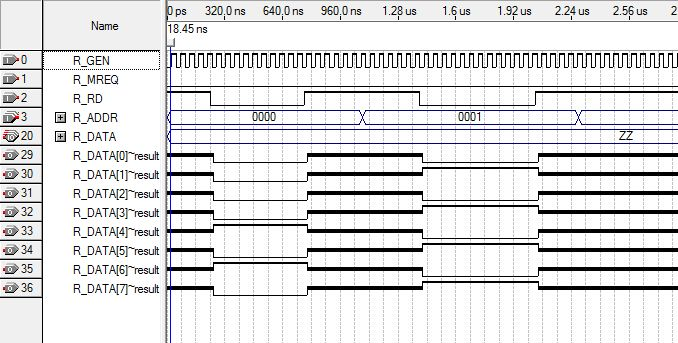
\includegraphics[width=15cm]{./pict/rom.jpg}
\caption{Przebiegi czasowe na poszczególnych liniach modułu pamięci ROM.}
\label{fig:rom}
\end{figure}

\section{Moduł operacji złożonej -- mnożenie Bootha}

Algorytm Bootha jest wykorzystywany do mnożenia dwóch liczb binarnych zapisanych w postaci U2.

Algorytm polega na sukcesywnym dodawaniu do sumy częściowej P jednej z dwóch predefiniowanych wartości -- A bądź S. Oznaczmy przez m i r mnożną i mnożnik naszego działania, a przez n ich ilość bitów.

\begin{enumerate}
  \item Ustalenie początkowych wartości A, S i P (każde z nich powinno być długości 2n+1 bitów)
  \begin{enumerate}
    \item Wypełnienie najstarszych n bitów liczby A wartością m, pozostałe bity zerujemy (A = \{m, 0..0\})
    \item Wypełnienie najstarszych n bitów liczby S wartością -m (w dopełnieniu do 2), pozostałe bity zerujemy (S = \{-m, 0..0\})
    \item Wypełniamy najstarsze bity P zerami, nastepnie wstawiamy liczbę r, a najmłodszy bit ustawiamy na 0 (P = \{0..0, r, 0\})
  \end{enumerate}
  \item Jeśli dwa najmłodsze bity sumy częściowej P wynoszą:
  \begin{enumerate}
    \item 01: P = P + A
    \item 10: P = P + S
    \item 00 lub 11: P pozostaje bez zmian
  \end{enumerate}
  \item Przesunięcie arytmetyczne P o jeden bit w prawo
  \item Powtórzenie kroków od 2 i 3 w sumie n razy
  \item Wynikiem mnożenia jest P po usunięciu najmłodszego bitu (przesunięciu bitowym w prawo)
\end{enumerate}

W projekcie mnożenie zostało zrealizowane jako osobny blok funkcjonalny, do którego podawane są mnożna i mnożnik. Blok ten posiada własny sygnał WAIT oznaczający trwające obliczenia, a po ich zakończeniu wynik jest udostępniany przy pomocy odpowiednich sygnałów. Obie liczby na wejściu muszą być tej samej długości (w projekcie przyjęto n=8, ale łatwo jest to zmienić), wynik natomiast jest dwukrotnie dłuższy (ze względu na architekturę projektowanego mikrokontrolera odczytywane jest tylko 8 młodszych bitów).

\section{Moduł wejścia -- klawiatura PS/2}

Moduł odpowiada za komunikację układu z urządzeniami zewnętrznymi za pomocą portu PS2. Transmisja danych przychodzących synchronizowana jest poprzez zewnętrzny zegar (ok. 15 kHz) dostarczany przez urządzenie komunikujące się z układem. Wewnętrzna struktura modułu oparta jest o maszynę stanów taktowana wewnętrznym sygnałem (ok. 20 MHz).  Maszyna stanów bada kolejność wprowadzanych znaków, jeżeli jest poprawna, wprowadzana liczba konwertowana jest na U2. Konwersja odbywa się poprzez sumowanie odpowiednio przemnożonych kolejnych cyfr dziesiętnych wprowadzanej liczby i odpowiednie ustawienie bitu znaku, jeżeli liczba należy do przedziału [-128; 127]

\begin{figure}[h]
\centering
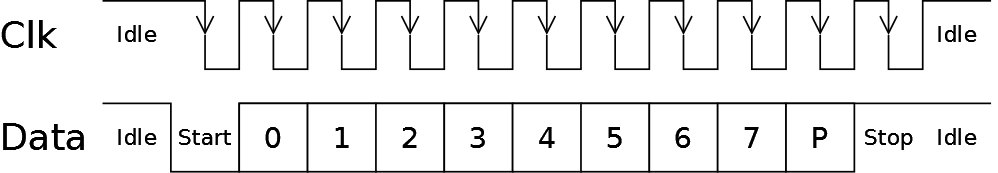
\includegraphics[width=8cm]{./pict/PS2.png}
\caption{Przebiegi czasowe na liniach portu PS/2 podczas transmisji pojedynczego znaku z klawiatury.}
\label{fig:ps2}
\end{figure}

\begin{figure}[h]
\centering
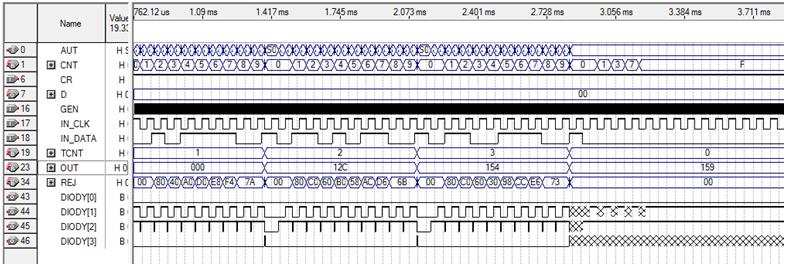
\includegraphics[width=11cm]{./pict/PS2_sim.png}
\caption{Przebiegi czasowe na liniach modułu PS2.}
\label{fig:ps2_sim}
\end{figure}

\section{Moduł wyjścia -- drukarka LPT}
Moduł odpowiada za komunikację z urządzeniami zewnętrznymi przy użyciu portu LPT. Moduł oparty jest o maszynę stanów taktowaną wewnętrznym zegarem (ok. 20 MHz). Poszczególne stany automatu odpowiadają etapom transmisji danych poprzez łącze równoległe. Moduł korzysta z opisanego poniżej modułu służącego do konwersji liczb z postaci U2 do BCD. Transmisja danych opiera się o wystawianie i utrzymywanie sygnałów sterujących zgodnie wymogami czasowymi transmisjiu~\ref{fig:lpt} , a także badanie stanu linii sterujących wejściowych. Moduł dokonuje także zamiany poszczególnych znaków liczby w postaci BCD na ich odpowiedniki w kodzie ASCII, którą są następnie wysyłane do urządzenia zewnętrznego (np. drukarki).

\begin{figure}[h]
\centering
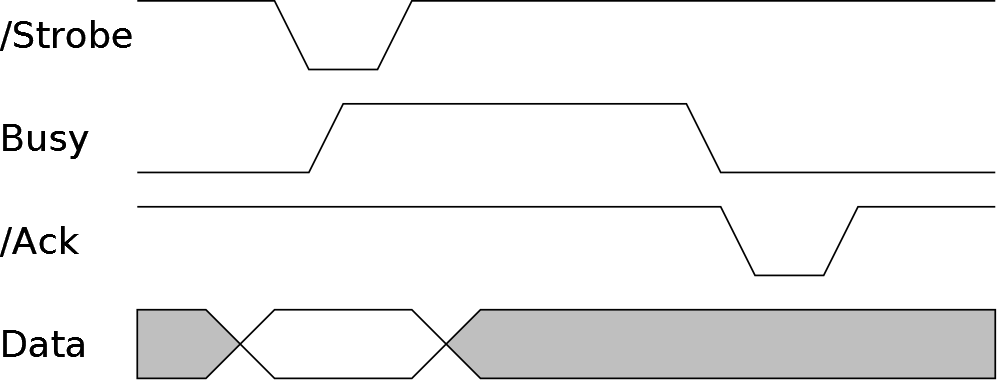
\includegraphics[width=8cm]{./pict/LPT.png}
\caption{Przebiegi czasowe na najważniejszych liniach portu LPT podczas wysyłania danych.}
\label{fig:lpt}
\end{figure}

\begin{figure}[h]
\centering
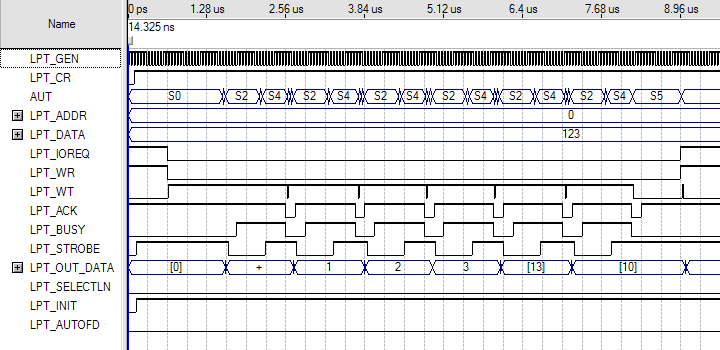
\includegraphics[width=11cm]{./pict/LPT_sim.png}
\caption{Przebiegi czasowe na liniach modułu LPT.}
\label{fig:lpt_sim}
\end{figure}

\subsection{Moduł zamiany liczb U2 na BCD}

Pierwszym krokiem konwersji liczb jest sprawdzenie i zapisanie znaku liczby w kodzie U2 i zamiana jej wartości bezwzględnej na liczbę w postaci NKB. Liczba z postaci NKB do postaci BCD konwertowana jest za pomocą algorytmu Shitf and Add 3 . Ogólna zasada działania algorytmu opiera się na stworzeniu bufora odpowiadającego sumarycznej wielkości znaków wyjściowych (u nasz 10 bit, po 4 bit na dziesiątki i jedności, 2 bity na cyfrę setek) i odpowiednim wsuwaniu z prawej strony liczby binarnej i testowaniu jej wartości. Jeżeli wartość kolumnie odpowiadającej którejś z cyfr liczby dziesiętnej jest większa bądź równa 5 to do tej kolumny dodajemy 3. Po wsunięciu wszystkich bitów konwertowanej liczby algorytm się kończy. W każdej z kolumn otrzymujemy wartość binarnie zapisaną wartość dziesiętną danej cyfry.

\section{Moduł testowy - wyświetlacz siedio segmentowy}
W czasie testowania stworzonego mikrokontrolera powstał jeszcze jedne dodatkowy moduł testowy. Pozwala on na wyprowadzanie na dwucyfrowy wyświetlacz 7-segmentowy aktualnej zawartości lini danych.

\begin{figure}[h]
\centering
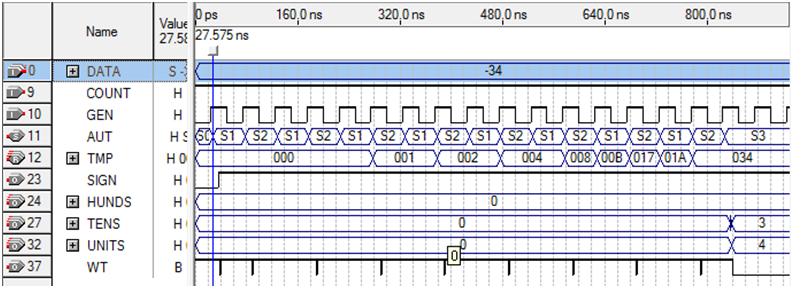
\includegraphics[width=11cm]{./pict/BCD_sim.png}
\caption{Przebiegi czasowe na liniach modułu LPT.}
\label{fig:lBCD_sim}
\end{figure}

%%%%%%%%%%%%%%%%%%%%%%%%%%%%%%%%%%%%%%%%%%%%%%%%
% Opis assemblera
%%%%%%%%%%%%%%%%%%%%%%%%%%%%%%%%%%%%%%%%%%%%%%%%
\chapter{Assembler}

\section{Opis}

W celu ułatwienia testowania układu stworzony został prosty program mający na celu tłumaczenie kodu programu z postaci źródeł assemblera na pliki .mif wczytywane przez program Quartus. Program, pomimo swojej prostoty, w znaczący sposób skrócił czas tworzenia programów testowych, a także wyeliminował potencjalne błędy mogące powstać podczas ręcznego uzupełniania zawartości ROMu.

Prostota programu nie oznacza jednak, że jest on bardzo ograniczony. Wręcz przeciwnie -- został napisany w sposób umożliwiający bardzo łatwe zaadaptowanie go do różnych architektur i zestawów instrukcji. Poprzez modyfikację pliku z definicją języka można zmienić długość kodów operacji, dodać nowe instrukcje, modyfikować ilość rejestrów wewnętrznych procesora, tworzyć nowe typy instrukcji (różne ilości i typy operandów).

\section{Instrukcja użycia}

\subsection{Definicja języka}

Plik z definicją języka podzielony jest na 3 sekcje:
\begin{itemize}
  \item definicja instrukcji
  \item definicja rejestrów
  \item definicja typów instrukcji
\end{itemize}

Każdy z sektorów musi zaczynać się liczbą oznaczającą ilość jego wpisów, a cały plik nie powinien zawierać pustych linii. Każdy wpis powinien być umieszczony dokładnie w jednej linii.

\subsubsection{Definiowanie instrukcji}
Ogólna postać definicji pojedynczej instrukcji składa się z 3 części:
\begin{itemize}
  \item Kod operacji w postaci binarnej -- wstawiany jest bezpośrednio w pliku wynikowym. Jego długość nie jest okreslona, ale dla danego typu instrukcji powinna być stała (każda instrukcja powinna w sumie składać się z pełnych bajtów).
  \item Mnemonik instrukcji -- tekstowy odpowiednik instrukcji używany w kodach źródłowych, podczas parsowania zastępowany odpowiednim kodem.
  \item Typ instrukcji -- jeden z typów określonych w 3 sekcji pliku z definicją języka. Określa ilość i typy parametrów dla danej instrukcji.
\end{itemize}

\subsubsection{Rejestry procesora}

W drugiej sekcji zawarta jest prosta definicja rejestrów dostepnych dla danej architektury. Każda linia składa się z nazwy symbolicznej rejestru i następujągo po niej binarnego kodu daneg rejestru (który wykorzystywany jest podczas tworzenia pliku wynikowego jako część instrukcji).

\subsubsection{Definiowanie typów instrukcji}

Trzecia sekcja pliku z definicją języka zawiera zdefiniowane typy instrukcji (do nich własnie odnoszą się typy z sekcji pierwszej). Każdy typ składa się z 2 głównych części: liczbiwego kodu typu oraz definicji składni instrukcji danego typu.

Definicja składni może zawierać jeden bądź wiele elementów składowych, z których kazdy oznacza, jak wynikowo powinna zostać złozona instrukcja, a także jakiego typu parametry są dozwolone. Możliwe wartości do wstawienia w tym miejscu to:
\begin{description}
  \item[OPCODE] -- kod instrukcji (mnemonik w kodzie źródłowym, binarny kod operacji w pliku wynikowym)
  \item[Rd] -- symboliczna nazwa jednego z rejestrów, zamieniana na jego kod w pliku wynikowym
  \item[IM8] -- liczba całkowita (w postaci dziesiętnej bądź szesnastkowej poprzedzonej '0x'), w pliku wynikowym zapisywana w postaci 8-bitowej
  \item[IM16] -- jak IM8, tyle że w pliku wynikowym zamieniana na liczbę 16-bitową
  \item[0] -- w tym miejscu w pliku wynikowym zostanie wstawione jedno 0, nie wpływa na postać instrukcji w kodzie źródłowym. Używane do wyrównywania instrukcji do wielokrotności 8 bitów.
\end{description}

\subsection{Pliki źródłowe}

Format plików źródłowych jest dość prosty, podobny do standardowych plików assemblera. Instrukcje zapisywane są przy pomocy kodów określonych w definicji języka, argumenty oddzielone mogą być przecinkiem, spacją, tabulatorem bądź dowolną ich kombinacją. 

Komentarze dostępne są jedynie w wersji całej linii (linia komentarza powinna zaczynać się od średnika). Wszystkie komentarze umieszczone na początku pliku przed pierwszą linią z kodem bądź przed pierwszą pustą linią są umieszczane na początku pliku wynikowego, pozostałe komentarze umieszczane są w pliku wynikowym bezpośrednio przed kodem wygenerowanym z następnej instrukcji.

\subsection{Kompilacja}

\section{Przykłady}

\label{sec:asmex}
\subsubsection{Assembler dla procesora z projektu}
\lstset{
tabsize=6
}\begin{lstlisting}[caption=Definicja języka,language=]

14
00000	STOP	0
00001	RESET	0
00010	JMP	1
00011	JZ	2
00100	ADD	3
00101	SUB	3
00110	LD	3
01000	OR	3
01001	AND	3
01010	LDI	2
01011	IN	2
01100	OUT	2
01110	STORE	4
10100	MUL	3
8
R0	000
R1	001
R2	010
R3	011
R4	100
R5	101
R6	110
R7	111
5
0	OPCODE 0 0 0
1	OPCODE 0 0 0 IM8
2	OPCODE Rd IM8
3	OPCODE Rd 0 Rd 0 Rd
4	OPCODE Rd IM16
\end{lstlisting}

Dostępnych jest 14 instrukcji 5 typów, każda z nich ma 5-bitowy kod. Procesor wyposażony jest w 8 rejestrów, każdy z nich o 3-bitowym kodzie. Typy instrukcji można przetłumaczyć następująco:
\begin{enumerate}
\setcounter{enumi}{-1}
  \item instrukcja składa się jedynie z samego kodu operacji, pozostałe zera służą do dopełnienia długości kodu wynikowego do wielokrotności 8 bitów. Instrukcja bezargumentowa.

  Przykład: STOP -- zatrzymanie wykonywania programu
  \item instrukcja posiadająca jeden argument typu całkowitoliczbowego, 8 bitowego. 

  Przykład: JMP 0x20 -- skok bezwarunkowy pod podany adres
  \item instrukcja posiadająca dwa argumenty -- w kolejności symbol rejestru oraz stałą liczbową 8-bitową.
  
  Przykład: LDI R3, -123 -- załadowanie do rejestru R3 wartości -123
  \item instrukcja posiadająca 3 argumenty, wszystkie będące symbolami rejestrów.

  Przykład: ADD R2, R3, R4 -- dodanie rejestrów R3 i R4, umieszczenie wyniku w rejestrze R2
  \item instrukcja posiadająca dwa argumenty - symbol rejestru oraz stała liczbową 16-bitową.

  Przykład: STORE R5, 0x1234 -- zapisanie wartości rejestru R5 do pamięci RAM pod adres 0x1234.
\end{enumerate}


\lstset{
tabsize=6,
morekeywords={IN, ADD, OUT, MUL}
}
\begin{lstlisting}[caption=Przykładowy kod programu,label=asm_1,language=oasm]
; Simple test program for VHDL general-purpose CPU
; Authors:
; 	Maciej Stefanczyk
;	Kacper Szkudlarek

	IN	R0, -1
	IN	R1, -1
	ADD	R2, R1, R0
	OUT	R2, 0
	IN	R1, -1
	MUL	R3, R1, R2
	OUT	R3, 0

; stop operation
	STOP
\end{lstlisting}

\lstset{
tabsize=6
}
\begin{lstlisting}[caption=Plik wynikowy dla źródła z listingu~\ref{asm_1},language=ahdl]
-- Simple test program for VHDL general-purpose CPU
-- Authors:
-- 	Maciej Stefanczyk
--	Kacper Szkudlarek
WIDTH = 8;
DEPTH = 32;
ADDRESS_RADIX = DEC;
DATA_RADIX = BIN;

CONTENT BEGIN
-- 6: IN	R0, -1
	0 :	01011000;
	1 :	11111111;
-- 7: IN	R1, -1
	2 :	01011001;
	3 :	11111111;
-- 8: ADD R2, R1, R0
	4 :	00100010;
	5 :	00010000;
-- 9: OUT	R2, 0
	6 :	01100010;
	7 :	00000000;
-- 10: IN	R1, -1
	8 :	01011001;
	9 :	11111111;
-- 11: MUL	R3, R1, R2
	10 :	10100011;
	11 :	00010010;
-- 12: OUT	R3, 0
	12 :	01100011;
	13 :	00000000;
-- stop operation
-- 15: STOP
	14 :	00000000;
END;
\end{lstlisting}
\lstset{
tabsize=4
}

%%%%%%%%%%%%%%%%%%%%%%%%%%%%%%%%%%%%%%%%%%%%%%%%
% Kody źródłowe
%%%%%%%%%%%%%%%%%%%%%%%%%%%%%%%%%%%%%%%%%%%%%%%%
\chapter{Kody źródłowe}

\section{Mikrokontroler}
\lstinputlisting[language=vhdl,label=lst_ram,caption=cpu.vhd]{../HDL/cpu.vhd}
\lstinputlisting[language=vhdl,label=lst_ram,caption=ram.vhd]{../HDL/ram.vhd}
\lstinputlisting[language=vhdl,label=lst_ram,caption=rom.vhd]{../HDL/rom.vhd}
\lstinputlisting[language=vhdl,label=lst_ram,caption=booth\_multiply.vhd]{../HDL/booth_multiply.vhd}
\lstinputlisting[language=ahdl,label=lst_ram,caption=input\_ps2.tdf]{../HDL/input_ps2.tdf}
\lstinputlisting[language=ahdl,label=lst_ram,caption=output\_lpt.tdf]{../HDL/output_lpt.tdf}
\lstinputlisting[language=ahdl,label=lst_ram,caption=u2tobcd.tdf]{../HDL/u2tobcd.tdf}

\section{Assembler}
\lstinputlisting[language=c++,label=lst_asm,caption=asm.cpp]{../ASM/asm.cpp}


\end{document}
